\documentclass{article}
\usepackage[utf8]{inputenc}
\usepackage[T1]{fontenc}
\usepackage{booktabs}
\usepackage{graphicx}
\usepackage{hyperref}
\usepackage{xcolor}
\definecolor{validated}{HTML}{047857}
\definecolor{refuted}{HTML}{B91C1C}
\definecolor{inconclusive}{HTML}{9A3412}
\title{Empirical Proof Record: REFUTED}
\date{2026-05-16T17:05:19.333094+00:00}
\begin{document}
\maketitle
\section*{Empirical Proof Record --- \textcolor{refuted}{\textbf{REFUTED}}}
\textbf{Proof ID:} \texttt{776d02f2497a8c0c5fd50ca26c816f76\dots}\\
\textbf{Created:} 2026-05-16T17:05:19.333094+00:00
\subsection*{1. Claim}
\begin{quote}Under a concentrated immune siege of labelled adversarial inputs, Kimera's GWF blocks no more than 10\% of benign inputs (the architectural false-positive ceiling).\end{quote}
\begin{itemize}
\item \textbf{Operationalisation:} fraction of benign-labelled corpus records for which the GWF returns a blocking verdict
\item \textbf{Threshold:} \texttt{gwf\_false\_positive\_rate <= 0.1 fraction}
\item \textbf{H0:} GWF false-positive rate > 0.1
\item \textbf{H1:} GWF false-positive rate <= 0.1
\end{itemize}
\subsection*{2. Verdict}
\textcolor{refuted}{\textbf{REFUTED}} --- observed \texttt{1.0}\\
GWF blocked 500/500 benign (100.0\% false-positive) and 500/500 malicious (100.0\% detection); the gwf direct target has no other defense layers — full-stack rates equal the GWF rates; 1000 cycles, 0 adapter errors
\begin{figure}[h!]\centering
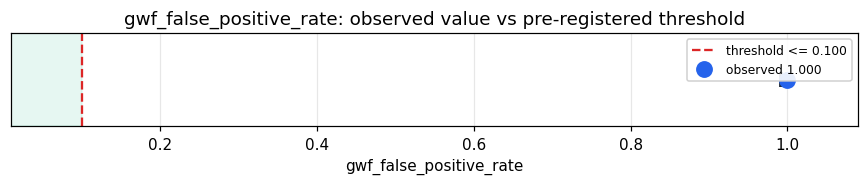
\includegraphics[width=0.8\linewidth]{assets/ci_gwf_false_positive_rate}
\caption{gwf\_false\_positive\_rate -- observed value with Wilson 95\% CI.}
\end{figure}
\subsection*{3. Evidence}
\begin{tabular}{llrrl}\toprule
\textbf{Pillar} & \textbf{Statistic} & \textbf{Value} & \textbf{95\% CI} & \textbf{Library} \\\midrule
\texttt{O.immune.false\_positive} & \texttt{gwf\_false\_positive\_rate} & \texttt{1.0} & (0.9924, 1.0000) & statsmodels 0.14.6 \\
\texttt{O.immune.detection} & \texttt{gwf\_detection\_rate} & \texttt{1.0} & (0.9924, 1.0000) & statsmodels 0.14.6 \\
\texttt{O.immune.full\_stack\_false\_positive} & \texttt{full\_stack\_false\_positive\_rate} & \texttt{1.0} & (0.9924, 1.0000) & statsmodels 0.14.6 \\
\texttt{O.immune.full\_stack\_detection} & \texttt{full\_stack\_detection\_rate} & \texttt{1.0} & (0.9924, 1.0000) & statsmodels 0.14.6 \\
\bottomrule\end{tabular}
\subsection*{4. Pre-registration}
\begin{itemize}
\item Registered at: \texttt{2026-05-16T17:05:18.425543+00:00}
\item Config hash: \texttt{b05d57c08adb0a277235dd1a174a660c\dots}
\item Data hash: \texttt{83109a27c3df2a45b912398b969fa8f7\dots}
\end{itemize}
\subsection*{5. Signature}
\texttt{7d1d1e4563fe95119411dcda1fd7522af40b1109dd2084be2afbe1e9ee03a7bf}\\

\end{document}
